\documentclass[english]{article}
\usepackage[OT1]{fontenc}
\usepackage{geometry}
\geometry{verbose,tmargin=2.5cm,bmargin=2.5cm,lmargin=2.5cm,rmargin=2.5cm}
\usepackage{float}
\usepackage{graphicx}
\usepackage{babel}

\usepackage{tikz}
\usepackage{pgfplots}
\usepackage{circuitikz}
\usetikzlibrary{arrows, positioning, calc,shapes}
\usepackage{enumitem}
\usepackage{hyperref}
\usepackage{nameref}% Only if hyperref isn't loaded

\usepackage{caption}
\usepackage{subcaption}
\usepackage{float}

\usepackage{amsmath,amssymb}
\makeatletter
\newsavebox\myboxA
\newsavebox\myboxB
\newlength\mylenA

\newcommand*\xoverline[2][0.75]{%
    \sbox{\myboxA}{$\m@th#2$}%
    \setbox\myboxB\null% Phantom box
    \ht\myboxB=\ht\myboxA%
    \dp\myboxB=\dp\myboxA%
    \wd\myboxB=#1\wd\myboxA% Scale phantom
    \sbox\myboxB{$\m@th\overline{\copy\myboxB}$}%  Overlined phantom
    \setlength\mylenA{\the\wd\myboxA}%   calc width diff
    \addtolength\mylenA{-\the\wd\myboxB}%
    \ifdim\wd\myboxB<\wd\myboxA%
       \rlap{\hskip 0.5\mylenA\usebox\myboxB}{\usebox\myboxA}%
    \else
        \hskip -0.5\mylenA\rlap{\usebox\myboxA}{\hskip 0.5\mylenA\usebox\myboxB}%
    \fi}
    
\makeatletter


\begin{document}

\title{Design of digital integrated systems: optimization of a 16 bit Brent-Kung adder}
\author{Matthijs Van keirsbilck}

\maketitle

\section{Schematic and optimisation}

\subsection{Optimisation}

\begin{enumerate}
\item Architectural \label{itm:arch}

\begin{itemize}
\item To remove inverters from the critical path, as a first attempt, the DotProducts were replaced with equivalent NAND-based operators. This was quite easy to implement, as only one type of DotProduct was needed, and provided a significant increase in performance. 

\item In the top half of the structure, most DotProducts are full-size (both generate and propagate).
Lower down, the propagate signal is often not used, so some gates can be removed, leading to lower power. See figure \ref{simpleStructure}.

\begin{figure}[h!]
\centering
\begin{subfigure}{.5\textwidth}
  \centering
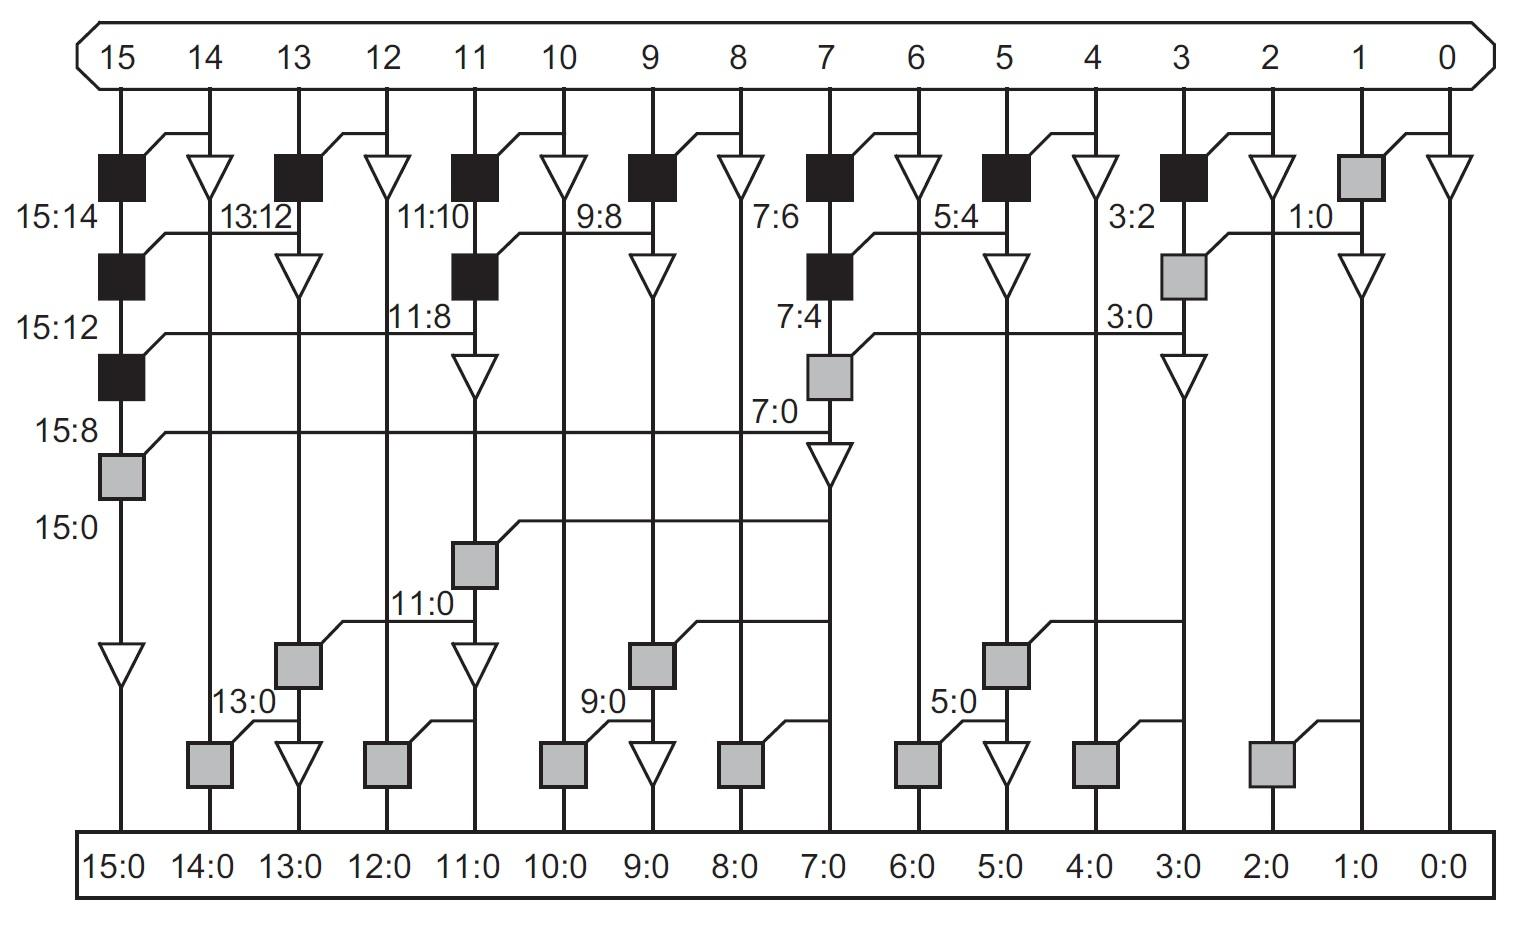
\includegraphics[width=0.9\textwidth]{figures/brentKungSimpleBlocksStructure}
\caption{Schematic of the adder with some simplified blocks. The buffers were left out in the implementation (see \ref{adderSchematic})}
\label{simpleStructure}
\end{subfigure}%
\begin{subfigure}{.5\textwidth}
  \centering
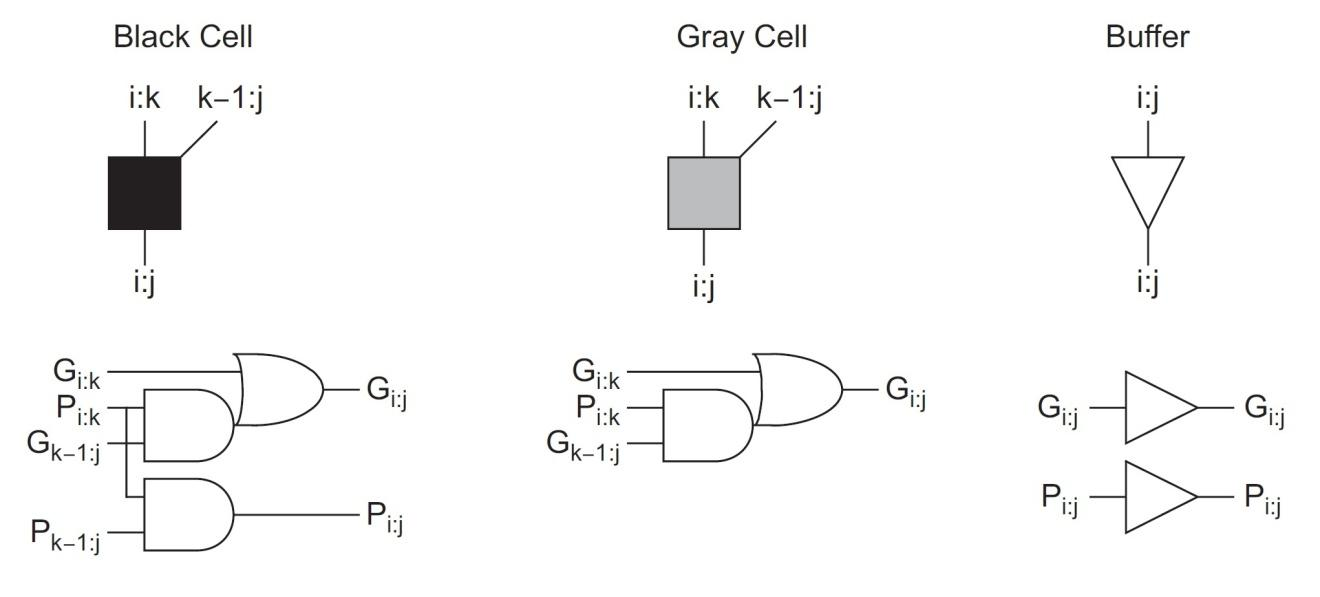
\includegraphics[width=0.9\textwidth]{figures/brentKungSimpleBlocks}
\caption{The structure of the blocks, with removed propagate generation where possible. \\ The buffers used in the final circuit only needed to buffer the generate signal.}
\label{simpleBlocks}
\end{subfigure}
\caption{Adder with some simplified blocks}
\end{figure}
  
\item Even better performance was reached by using AOI and OAI- based DotOperators, where the DotProducts are replaced with DotProductNormal and DotProductInverse. In the rest of the report, that architecture will be described.
As the number of normal/inverting stages is not equal for all paths, some special operators are required as well. DotProductSimpleNormalHighInvertedLow for example is a dotproduct that doesn't generate a propagate signal, and takes as input  $P_h$, $G_h$, and \xoverline{G_l}.\\
In total, there are six different DotOperators (with their abbreviations between brackets):

\begin{enumerate}
\item DotOperatorNormalIn ('DON')
\item DotOperatorInvertedIn ('DOI')
\item DotOperatorSimpleNormalIn ('DOSN')
\item DotOperatorSimpleInvertedIn ('DOSI')
\item DotOperatorSimpleNormalHighInvertedLow ('DOSNHIL')
\item DotOperatorSimpleInvertedHighNormalLow ('DOSIHNL')
\end{enumerate}
See section \ref{subsec:Schematics} and  the structural schematic (Figure \ref{adderSchematic}). \par
Some of the paths require an inverter before the XOR sum-generation. These paths therefore have longer delay. We can reduce this imbalance by scaling the invertor/XOR gates (see Sizing).

\item An efficient 6-transistor implementation of the XOR gate (based on transmission gates) decreases delay by a lot, because of less transistors, faster switching speed and reduced load on the critical path. Because only one consecutive transmission gate stage is used, output isn't degraded much and no buffers are needed (see reference \cite{website:xorTransmissionGate}).

\begin{figure}[H]
\begin{centering}
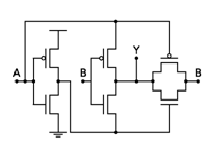
\includegraphics{figures/efficientXOR.png}
\par\end{centering}
\caption{Schematic of the optimised XOR gate}
\label{adderSchematic}
\end{figure}

\item If buffers in the structure buffer a large subcircuit, they will significantly reduce the load on critical path, making it faster. The buffers increase the delay of the path they are placed on, however. This could make those paths the new bottlenecks. \par
One buffer is located after DotOperator3\_0, to buffer s4-s7 away from the critical path. A simulation with a buffer after DotOperator1\_0 was run, but the extra load of the buffer compensated for the lower load on the critical path due to buffering, so it was left out. \par
The second buffer was introduced after DotOperator7\_0, but low in the hierarchy to prevent it from adding delay to the most critical paths to s15, s14, s13 and s11. \par
More buffers or buffers higher up in the hierarchy didn't improve speed, so were left out. See the structural schematic in Figure \ref{adderSchematic}.
\end{itemize} %end arch


\item Sizing \label{itm:sizing}

For achieving maximum speed, widths of some transistors were changed by some scalar factor:
\begin{itemize}
\item The building blocks (AOI, OAI, NAND, XOR, NOT) were optimized in size to take into account that some transistors were placed in parallel or in series, respectively increasing or reducing the current in that branch. See below.

\item pMOSscalar: normally, pMOS devices are sized about twice as large as nMos devices to keep switching symmetrical (this is needed due to lower mobility of holes compared to electron)s. For this adder design, however, lower pMOS width means lower capacitance, and this results in faster switching speeds. Too low values mean that the asymmetricalities will increase delay, too high values increase the capacitive load and reduce delay as well. This trade-off resulted in an optimal pMOS sizing of 1.6 times the nMOS size for maximum speed. \\
A pMOS scaling of 1 results in lower EDP however, so for the power optimization with a delay constraint of 650ps, it's better to use minimum size transistors.

\item seriesScalar: for example in a NAND gate, the 2 nMOS devices are placed in series between output and ground. This results in higher series resistance for the current flow and an extra capacitive node that needs to be drained. Series devices can provide less current than a single device due to these reasons, while devices in parallel can provide double the current. To compensate for these effects, transistors in series configurations are scaled by a factor of seriesScalar.

\item critBasePath: The top right quarter of the adder (from input0 to input7, and down to DotOperator(7\_0)) is quite important for all critical paths. This scalar modifies the widths of transistors in this area.

\item critPath1: The second half of the most critical path (6 DotOperators), running diagonally from DotOperator(7\_0)) to s15. Increasing its size improves speed, but also increases loading.

\item critPath2: The secondmost critical path. If the first critical path is sized large enough, it will no longer have the largest delay, and this second critical path needs to be scaled as well. This increases the load on the first critical path, increasing its delay. A balance needs to be found.

\item XORScalar: some of the paths are more critical than others. For precise adjustments to the path delay, the XOR gates at the end of the path can work faster if they are scaled, without increasing the sizing of the whole path (which would have a large effect on the loading as well). The most important paths at s15 and s9, as well as s14 and s13 were scaled this way.

\item VDD: this reduces the DC power consumtion and the switching energy, but increases the delay. When a good Energy-Delay Product (EDP) is reached, scaling the voltage reduces power consumption. Vdd= 0.938V was the lowest supply voltage where the circuit still fulfilled the specifications.

\end{itemize} % end sizing

\end{enumerate} %end architectural/sizing 



\section{Results} \label{sec:Results}
Two different circuits are shown, one that targets maximum possible speed, and another that targets minimum power with a delay constraint of 650ps.
To measure these results properly and determine worst-case performance, one test file was run for each path (thanks to Bob Vanhoof for providing some basic test files). 
The shown delay, switching energy, and EDP are the worst (maximum) delay of all test cases (not necessarily the same one). The DC power obviously remains constant for a given architecture.
Observing delays for all paths lead to guesstimates for sizing. The optimal sizing was determined by iteratively improving the scalars described in section (see section \ref{itm:sizing}).

\subsection{Maximum speed}
\begin{table}[h]
\centering
\begin{tabular}{ |l|r| }
\hline
scalar	& value \\
\hline
 pMOSscalar		& 1.6 \\
 seriesScalar   & 2.6 \\
 critBase   	& 1.0 \\
 critPath1   	& 1.89 \\
 critPath2    	& 1.0 \\
\hline
\end{tabular}
\caption{Size Scaling factors for maximum speed}
\label{SpeedScalars}
\end{table}

\begin{table}[h]
\centering
\begin{tabular}{ |l|r| }
\hline
Supply						&	1 V \\
Worst Case delay &            507.8 ps  \\
Worst Case Switching energy & 135.26 fJ \\
Worst Case DC power &         1.73   nW  \\
Worst Case EDP &              68660 ps*fJ \\
\hline
\end{tabular}
\caption{Performance of the circuit tuned for maximum speed}
\label{SpeedPerformance}
\end{table}


\subsection{Minimum EDP and Power at 650ps delay}

For the maximum speed circuit, the delay goes up when pMOSscalar is lowered too much, but this is not the case for the minimum power circuit (the only difference between the circuits is the sizing of the critical paths).\par
	For the minimum power circuit, it is a bit surprising that the extremely low (minimal sizing) width of pMOS transistors compared to nMOS doesn't increase delay (since it introduces asymmetricalities). Instead, this sizing improves the EDP of the adder by a large margin (EDP of 55k while it was $>$ 70k for the maximum speed).\par
As an illustration, see Table \ref{PowerPerformancePMOS1.6}. If pMOS transistors are sized at 1.6 * nMos\_sizing, then speed is increased and VDD can be lowered down to 0.926V. However, the power consumption of this circuit is considerably worse in than the minimal size circuit as transistors are much larger. \par
Another illustration is shown in Table \ref{bestEDP}. Maximum EDP is obtained for a pMOS scaling of 1, and supply voltage of 1V. This makes sense since EDP doesn't into account the DC power consumption, which is influenced most by VDD variations.

\begin{table}[h]
\centering
\begin{tabular}{ |l|r| }
\hline
Supply	&	0.926 V \\
Worst Case delay &            648.95 ps \\
Worst Case Switching energy & 115.29 fJ \\
Worst Case DC power &         1.12 nW \\
Worst Case EDP &              74625.7193 ps*fJ \\
\hline
\end{tabular}
\caption{Performance for minimum power at 650ps delay, \\ with pMOSscalar = 1.6}
\label{PowerPerformancePMOS1.6}
\end{table}  

\begin{table}[h]
\centering
\begin{tabular}{ |l|r| }
\hline
Supply	&	1 V \\
Worst Case delay &            523 ps \\
Worst Case Switching energy & 99.54 fJ \\
Worst Case DC power &         1.49 nW \\
Worst Case EDP &              51792 ps*fJ \\
\hline
\end{tabular}
\caption{Performance for minimum EDP, \\ with pMOSscalar = 1.0 and VDD = 1V}
\label{bestEDP}
\end{table} 

\begin{table}[h]
\centering
\begin{tabular}{ |l|r| }
\hline
Supply	&	0.933 V \\
Worst Case delay &            648.2 ps \\
Worst Case Switching energy & 86.02 fJ \\
Worst Case DC power &         1.01 nW \\
Worst Case EDP &              55767 ps*fJ \\
\hline
\end{tabular}
\caption{Final Performance: minimum power at 650ps delay, \\ with pMOSscalar = 1.0 and VDD = 0.933V}
\label{PowerPerformancePmos1.0}
\end{table}  

\newpage{}


\subsection{Schematics} \label{subsec:Schematics}

\subsubsection{DotOperators}


\begin{figure}[h!]
\centering
\begin{subfigure}{.5\textwidth}
  \centering
  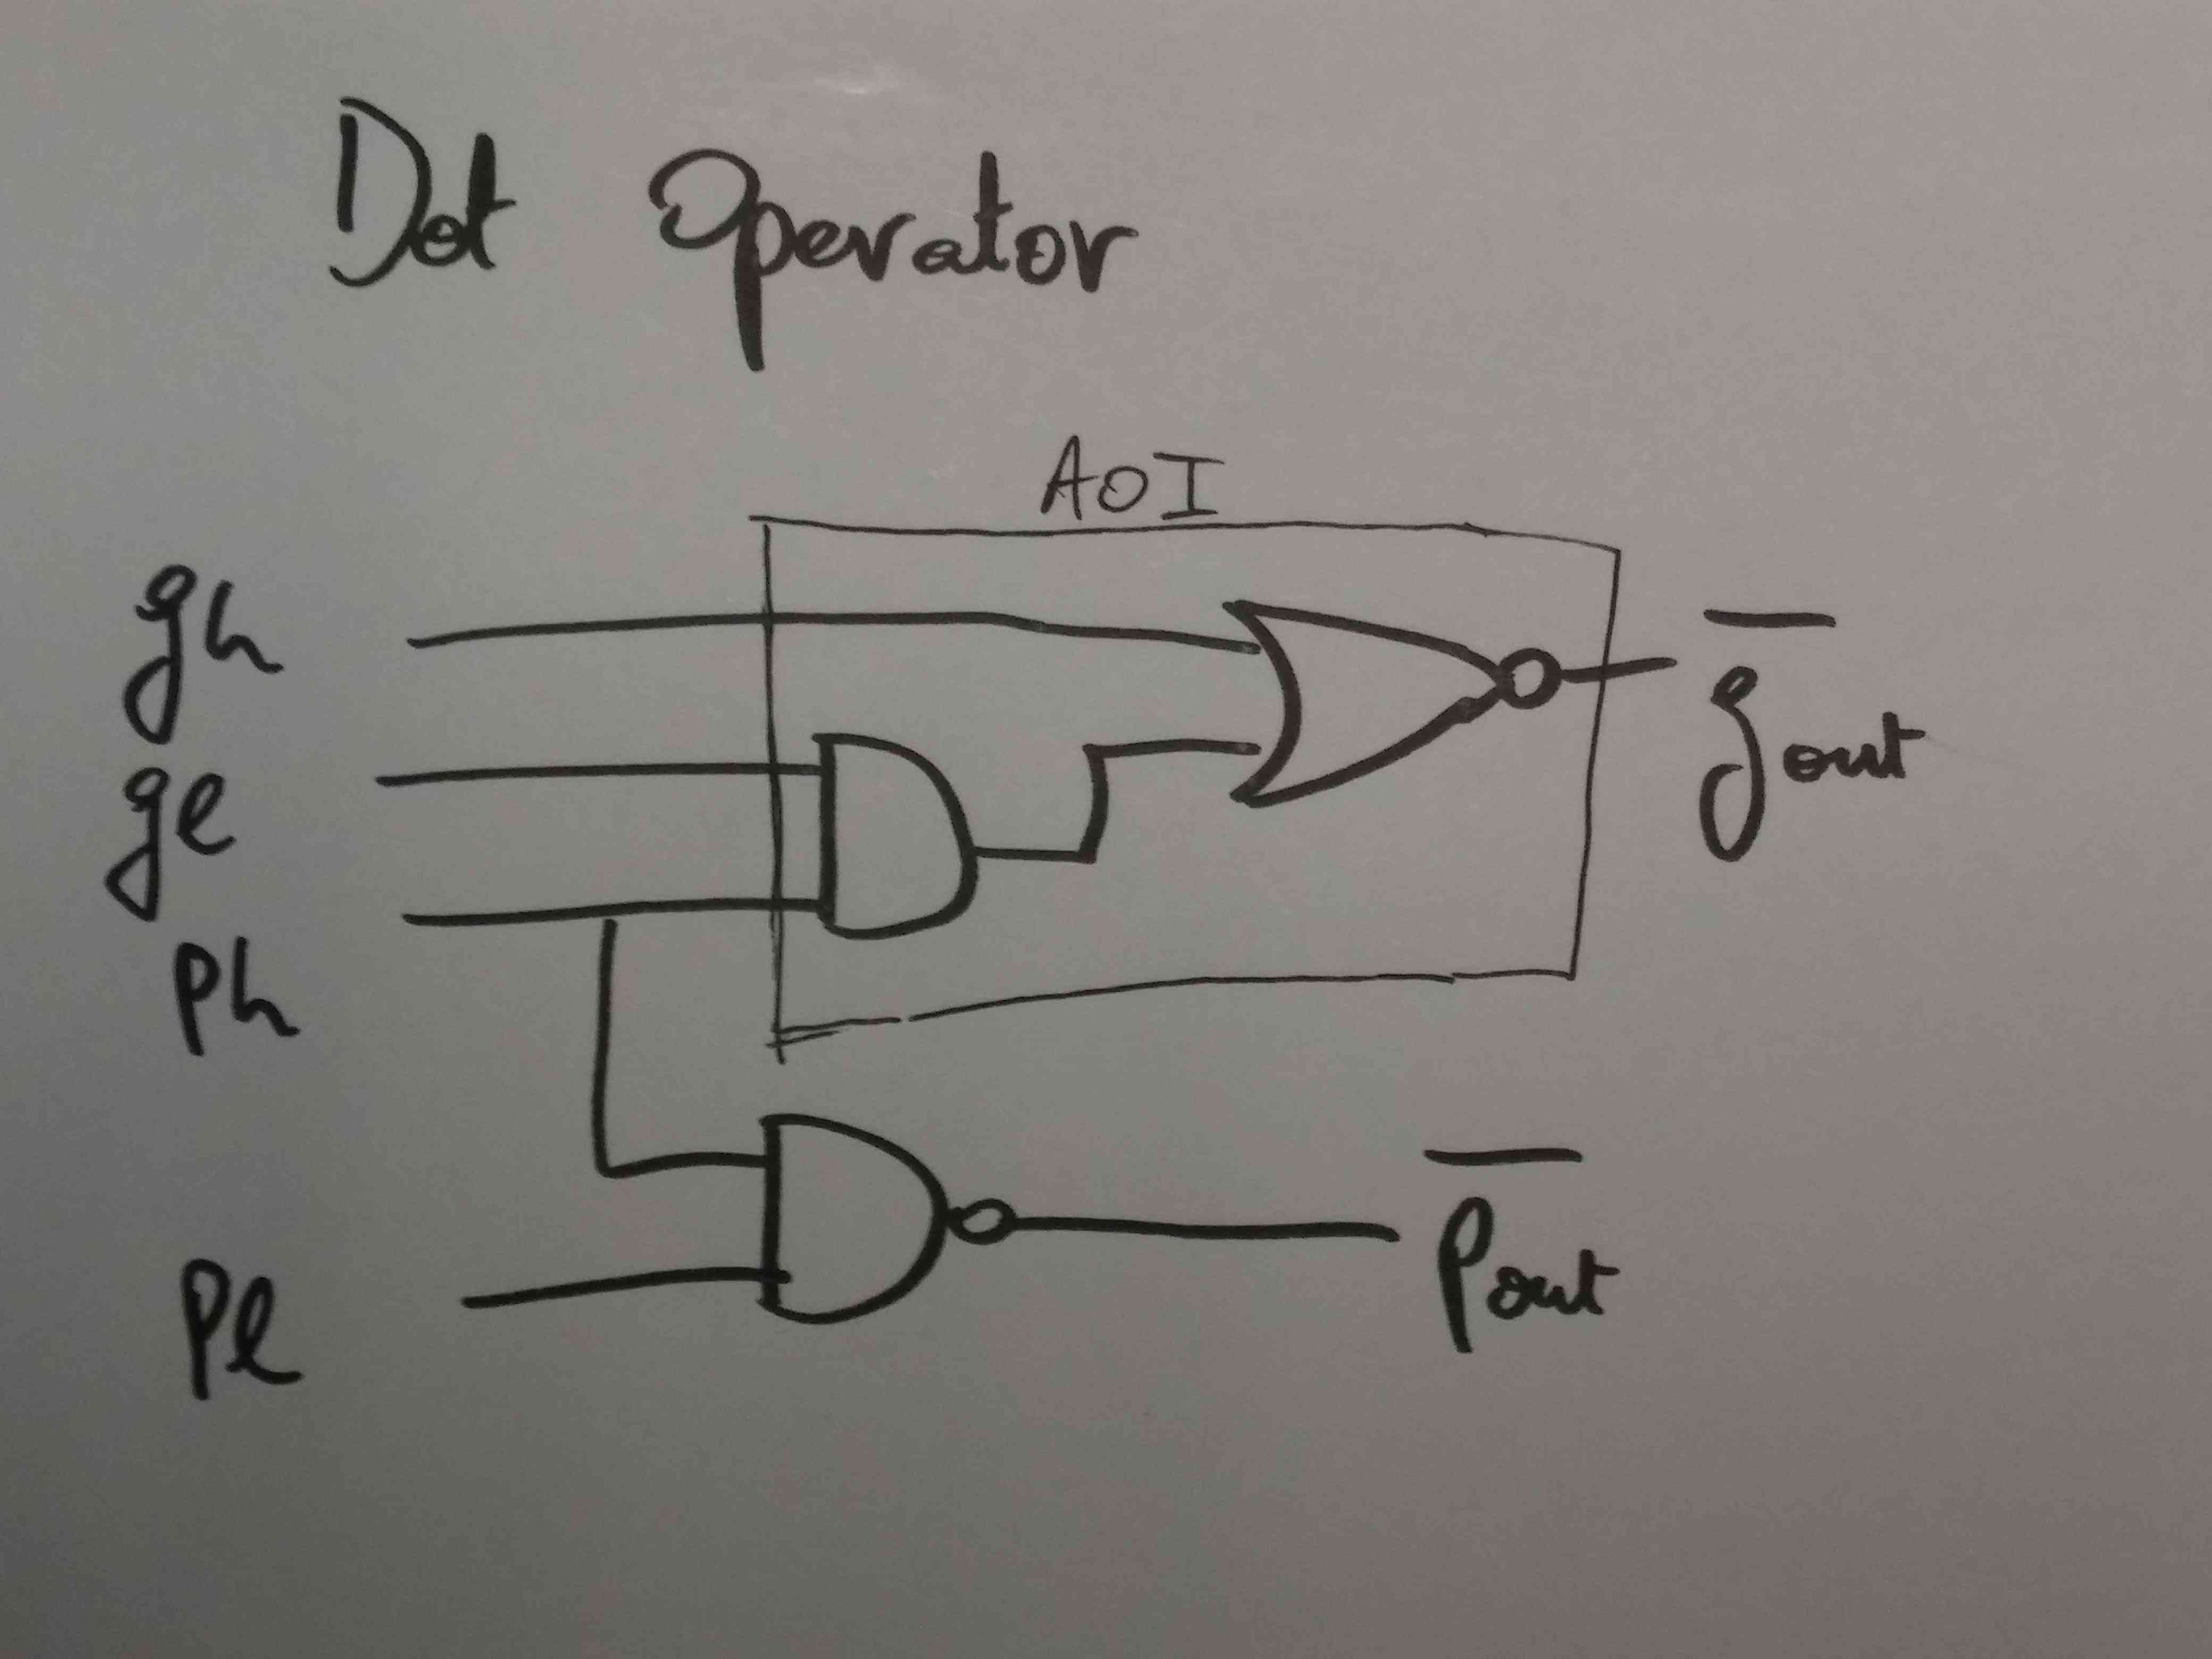
\includegraphics[width=0.9\textwidth]{figures/do}
\caption{the Dot Operator ('DO')}
\label{DO}
\end{subfigure}%
\begin{subfigure}{.5\textwidth}
  \centering
  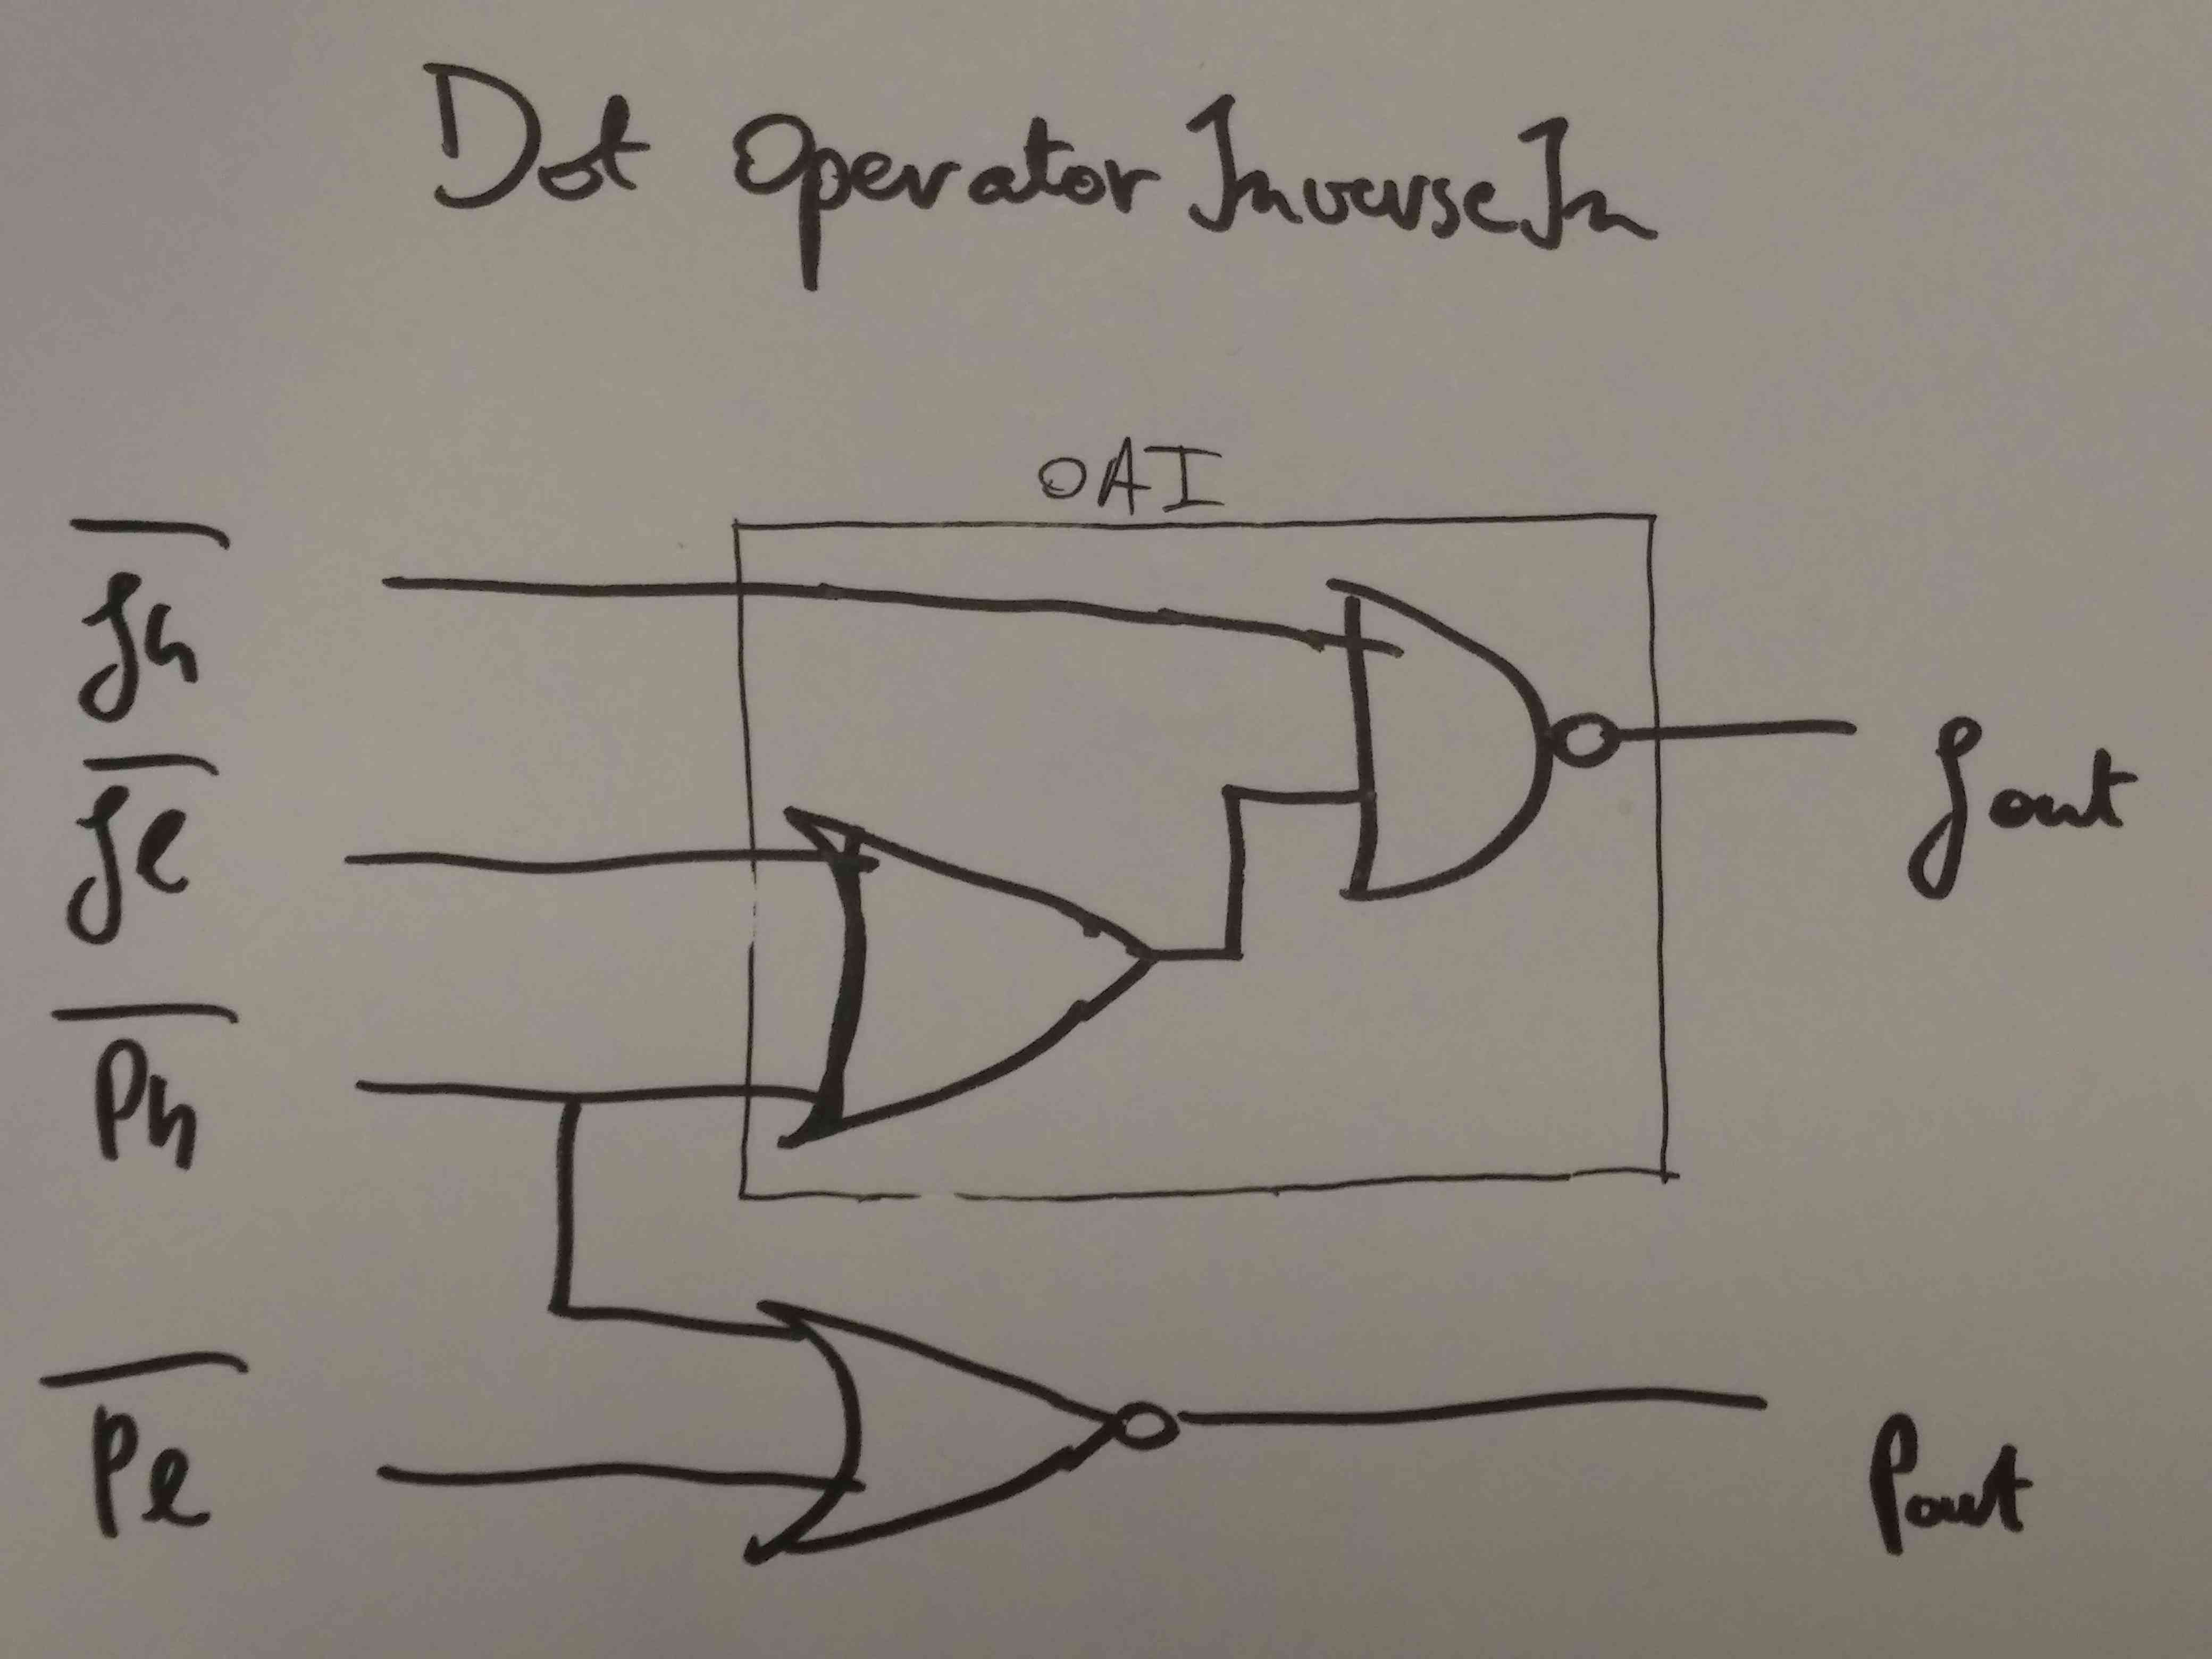
\includegraphics[width=0.9\textwidth]{figures/doi}
\caption{the Dot Operator with inverted inputs ('DOI')} 
\label{DOI}
\end{subfigure}
\end{figure}

\begin{figure}[h!]
\centering
\begin{subfigure}{.5\textwidth}
  \centering
  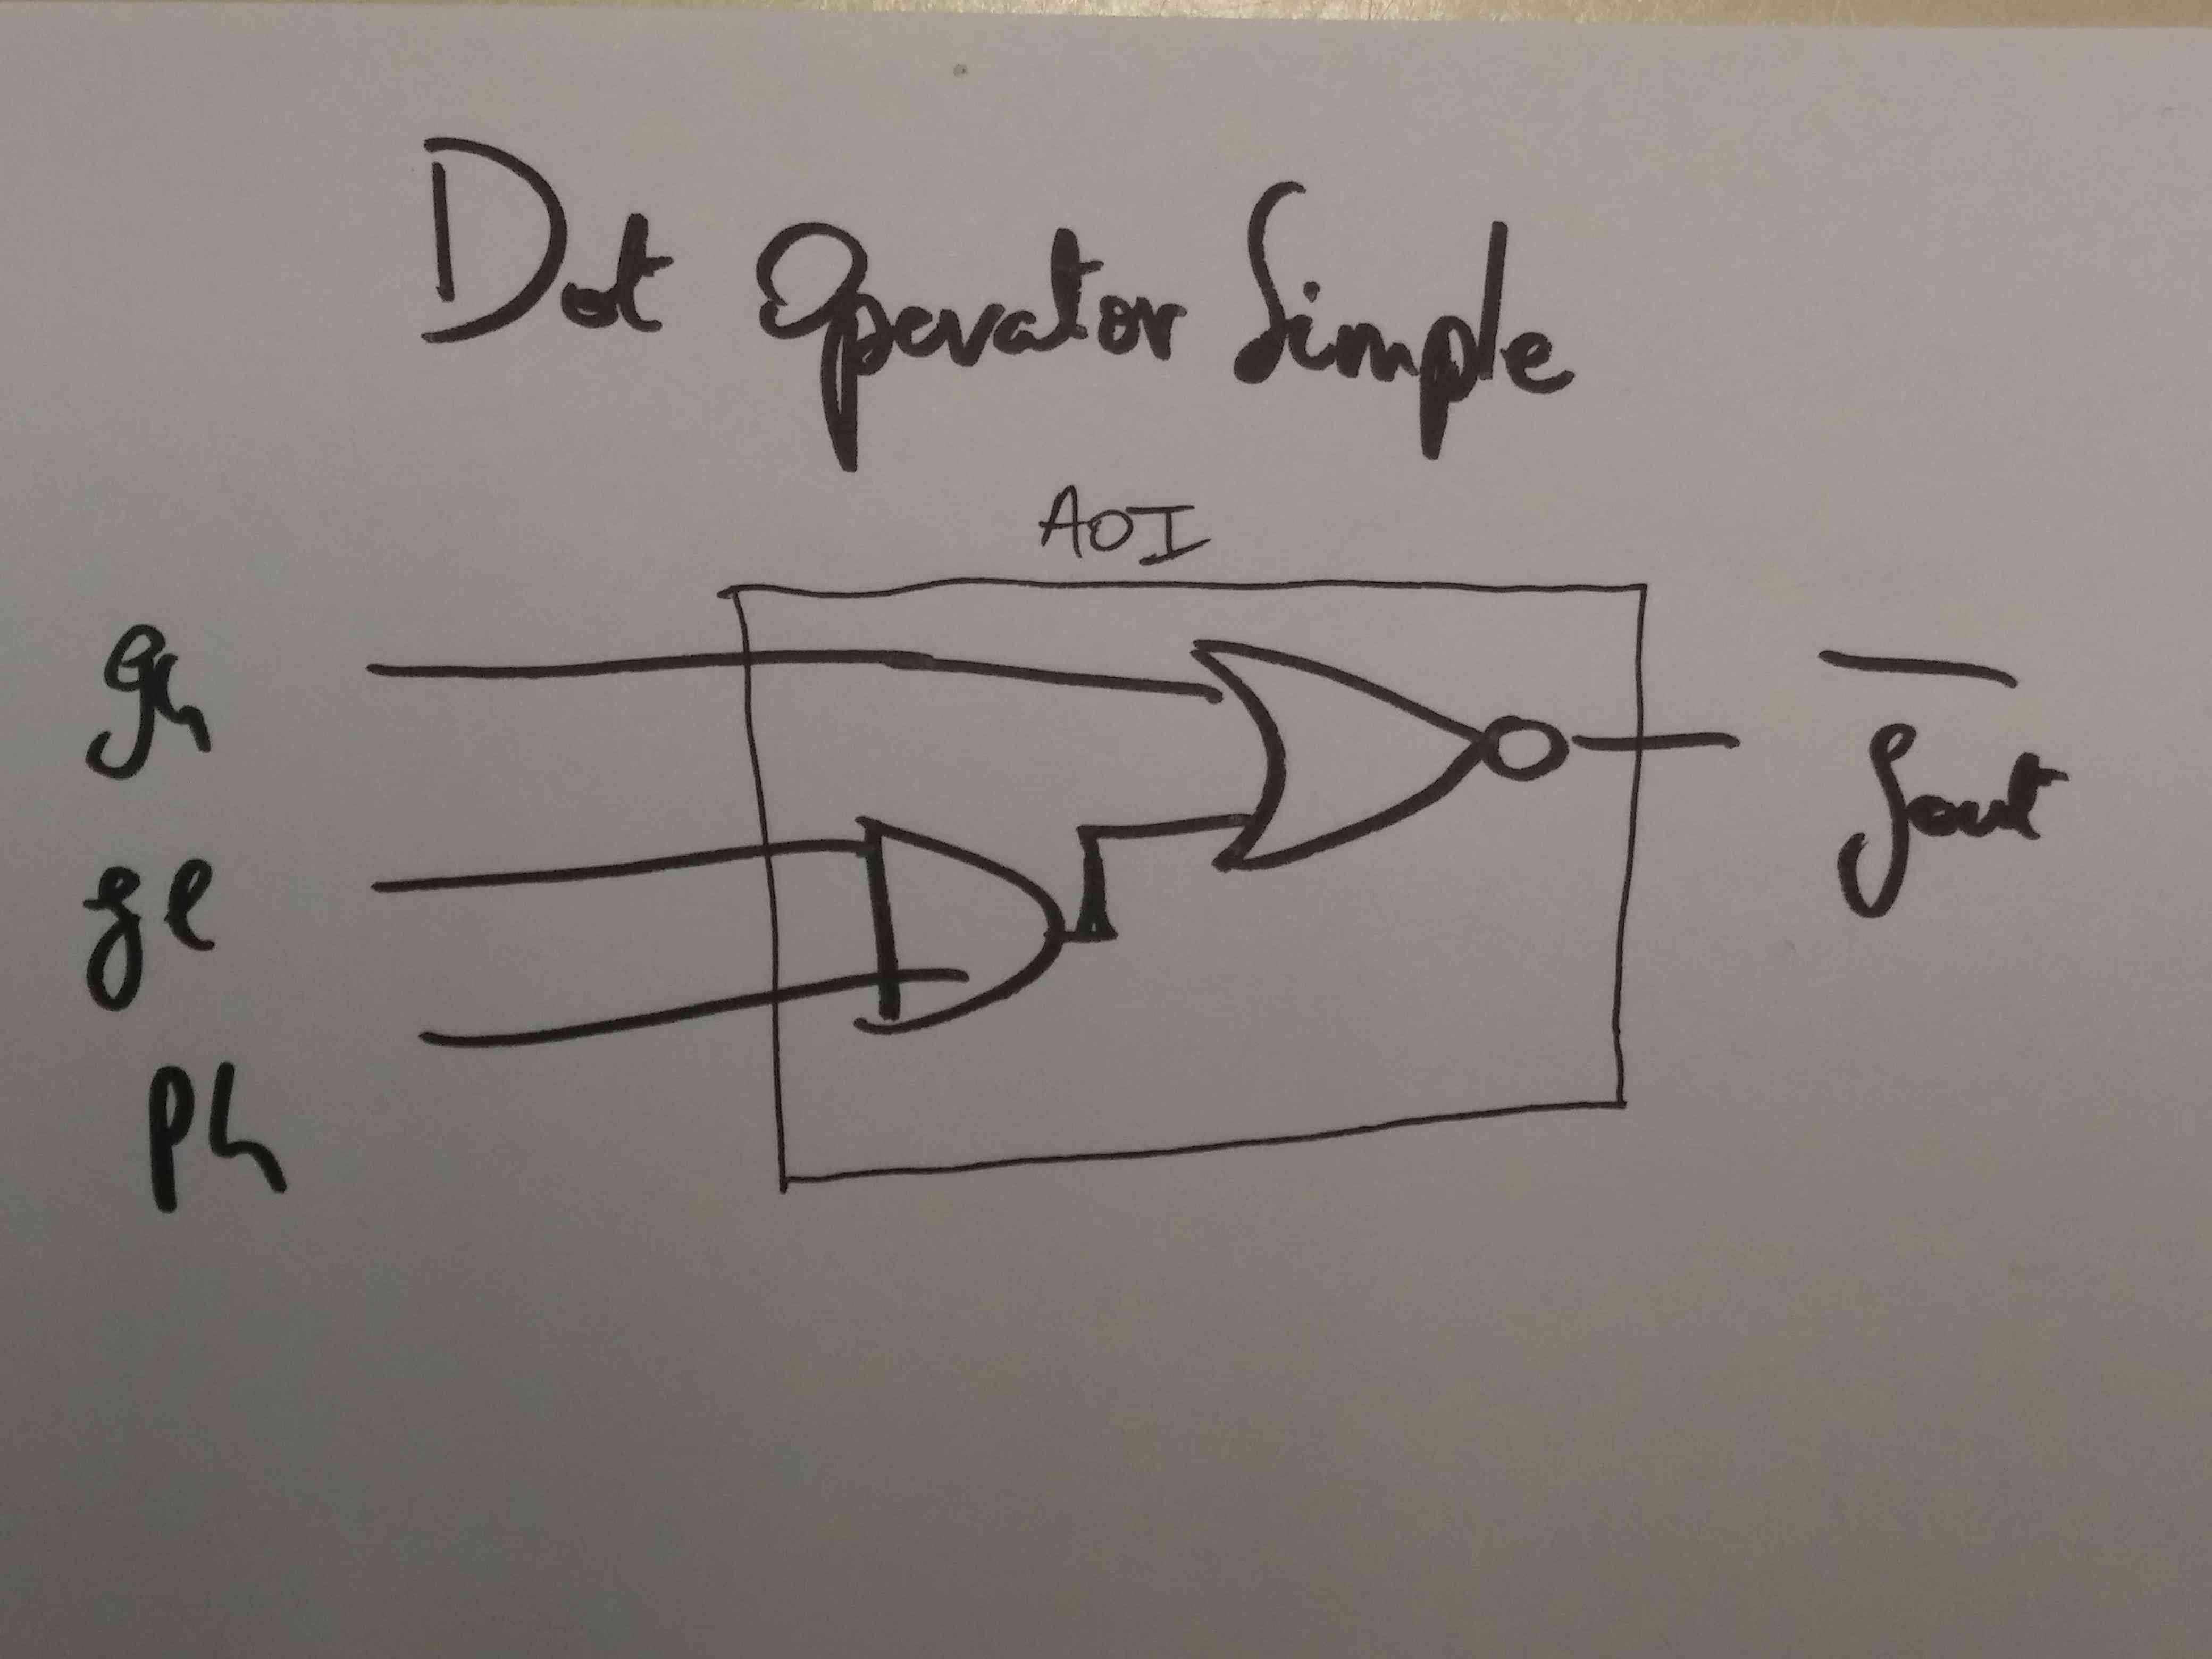
\includegraphics[width=0.9\textwidth]{figures/dos}
\caption{the Dot Operator Simple, \\without propagate generation ('DOS')}
\label{DOS}
\end{subfigure}%
\begin{subfigure}{.5\textwidth}
  \centering
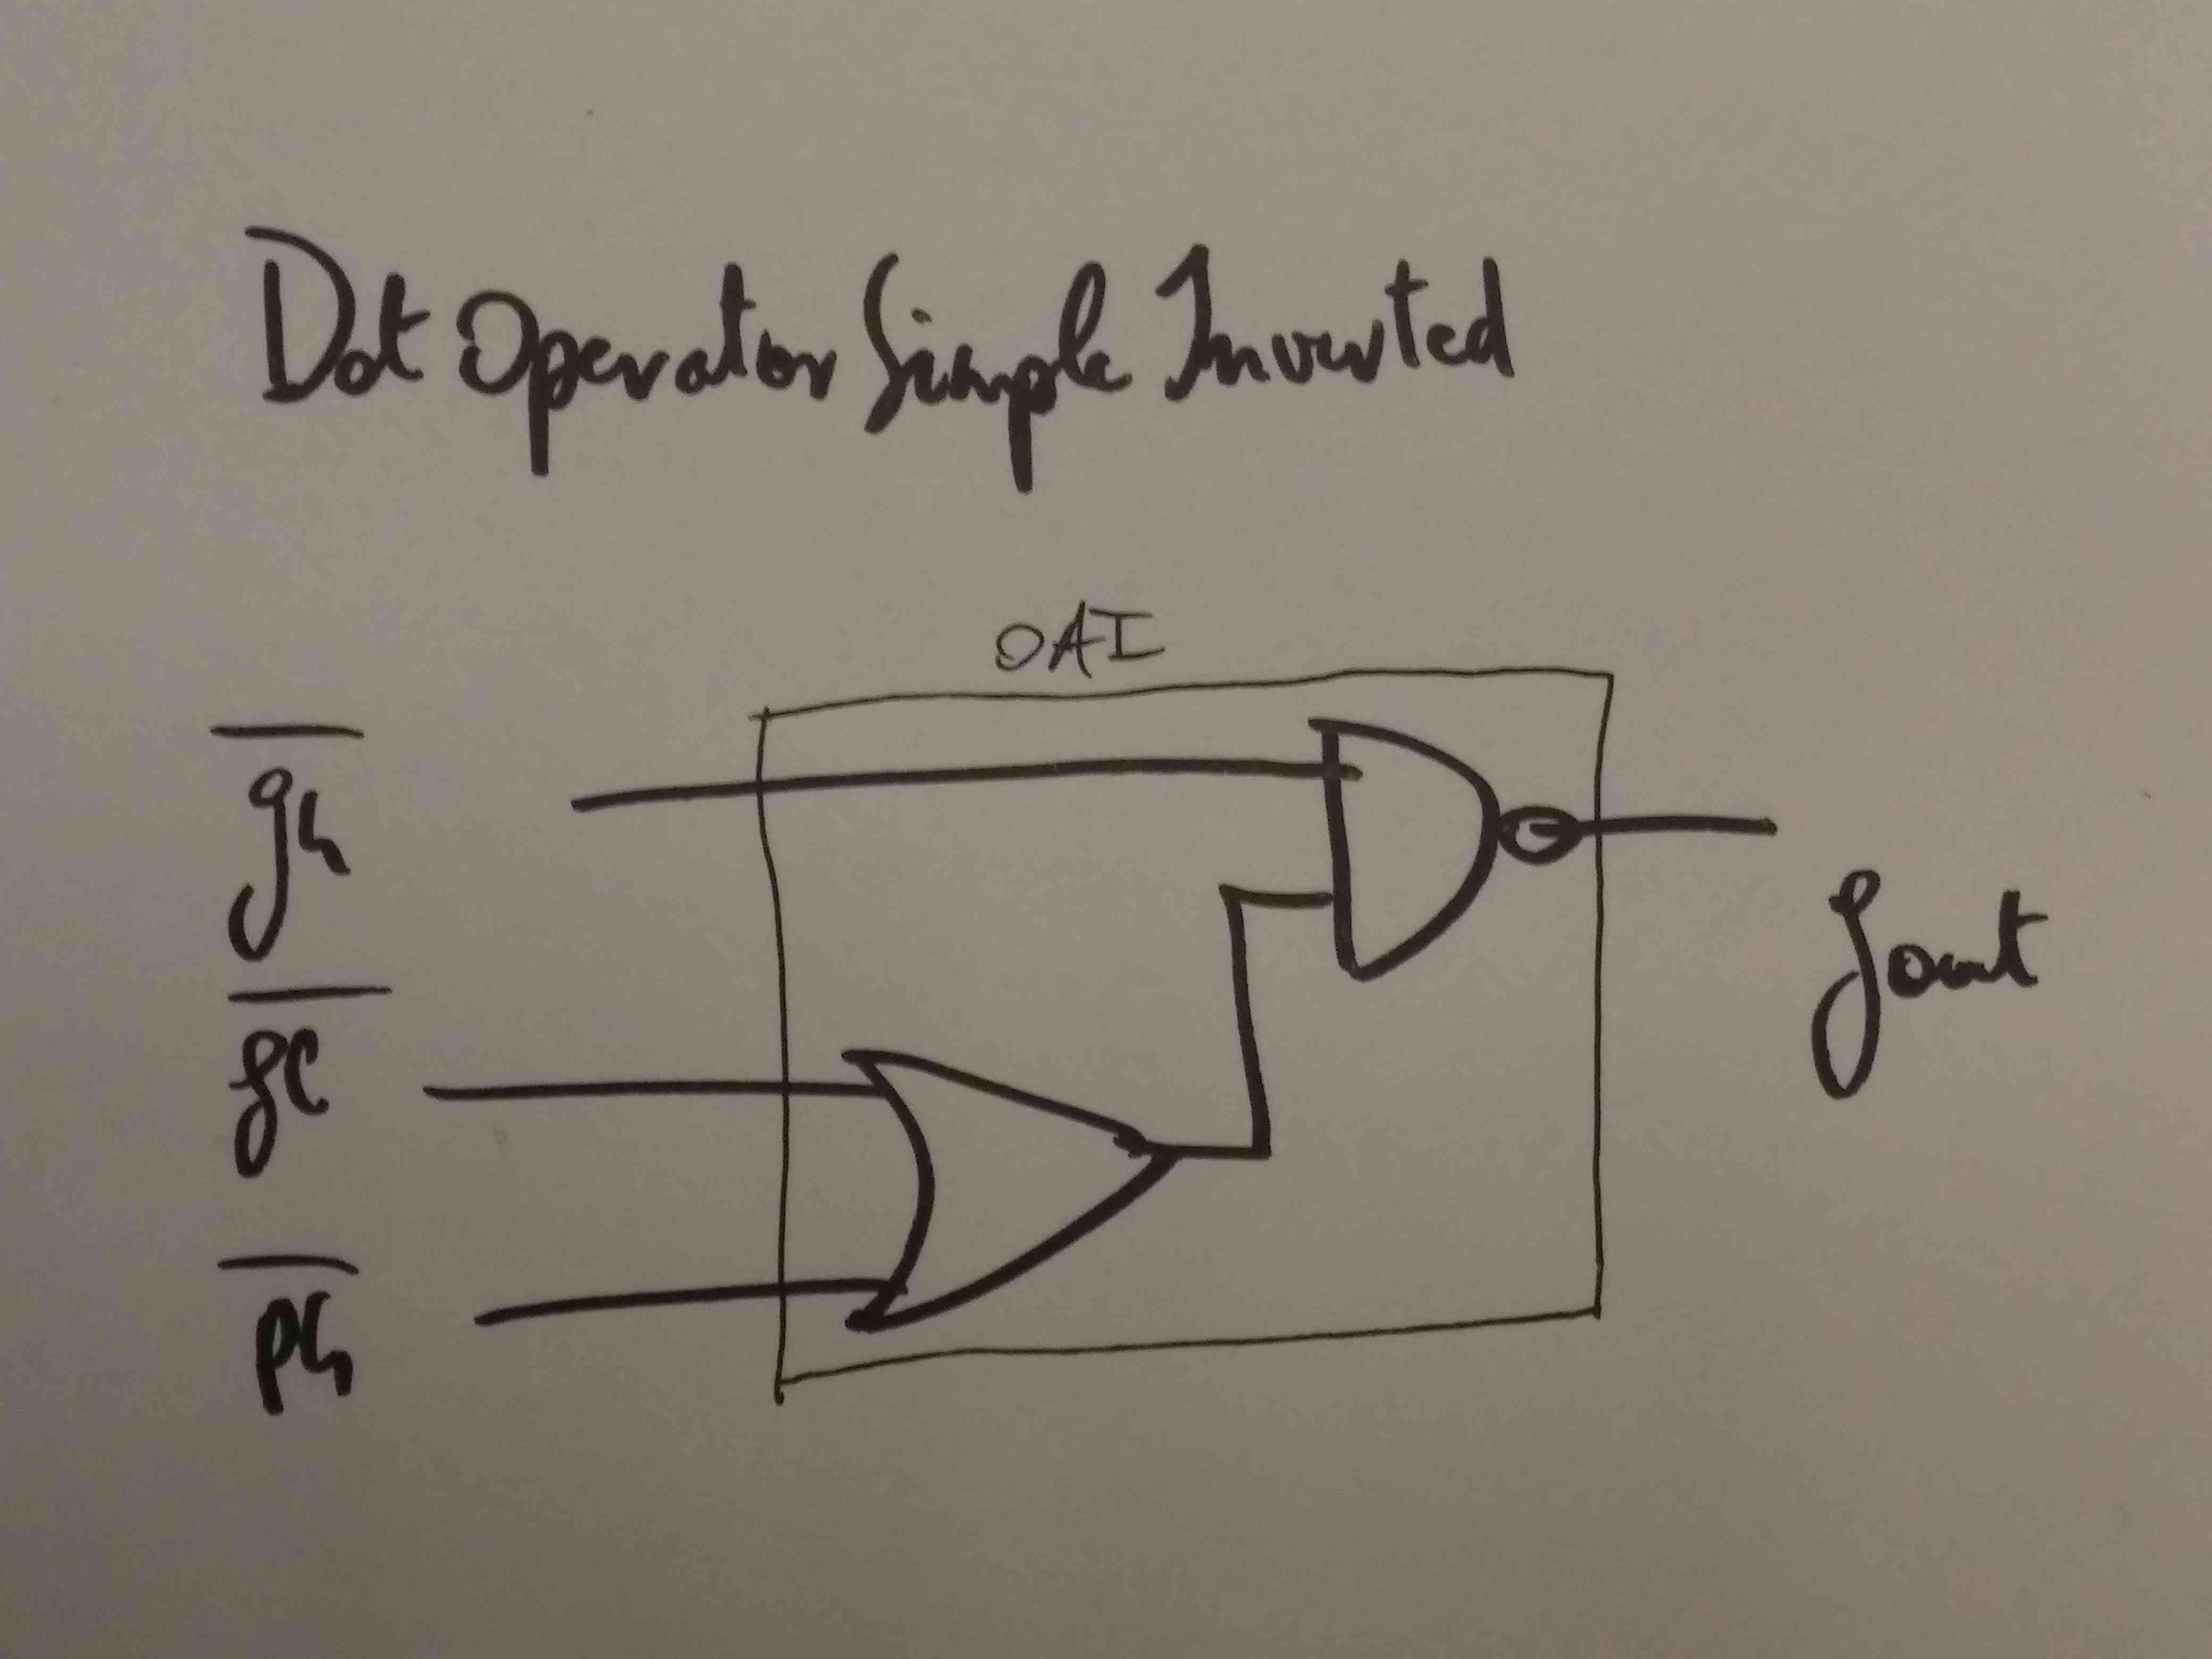
\includegraphics[width=0.9\textwidth]{figures/dosi}
\caption{the Dot Operator Simple, \\Inverted inputs ('DOSI')}
\label{DOSI}
\end{subfigure}
\end{figure}

\begin{figure}[h!]
\centering
\begin{subfigure}{.5\textwidth}
  \centering
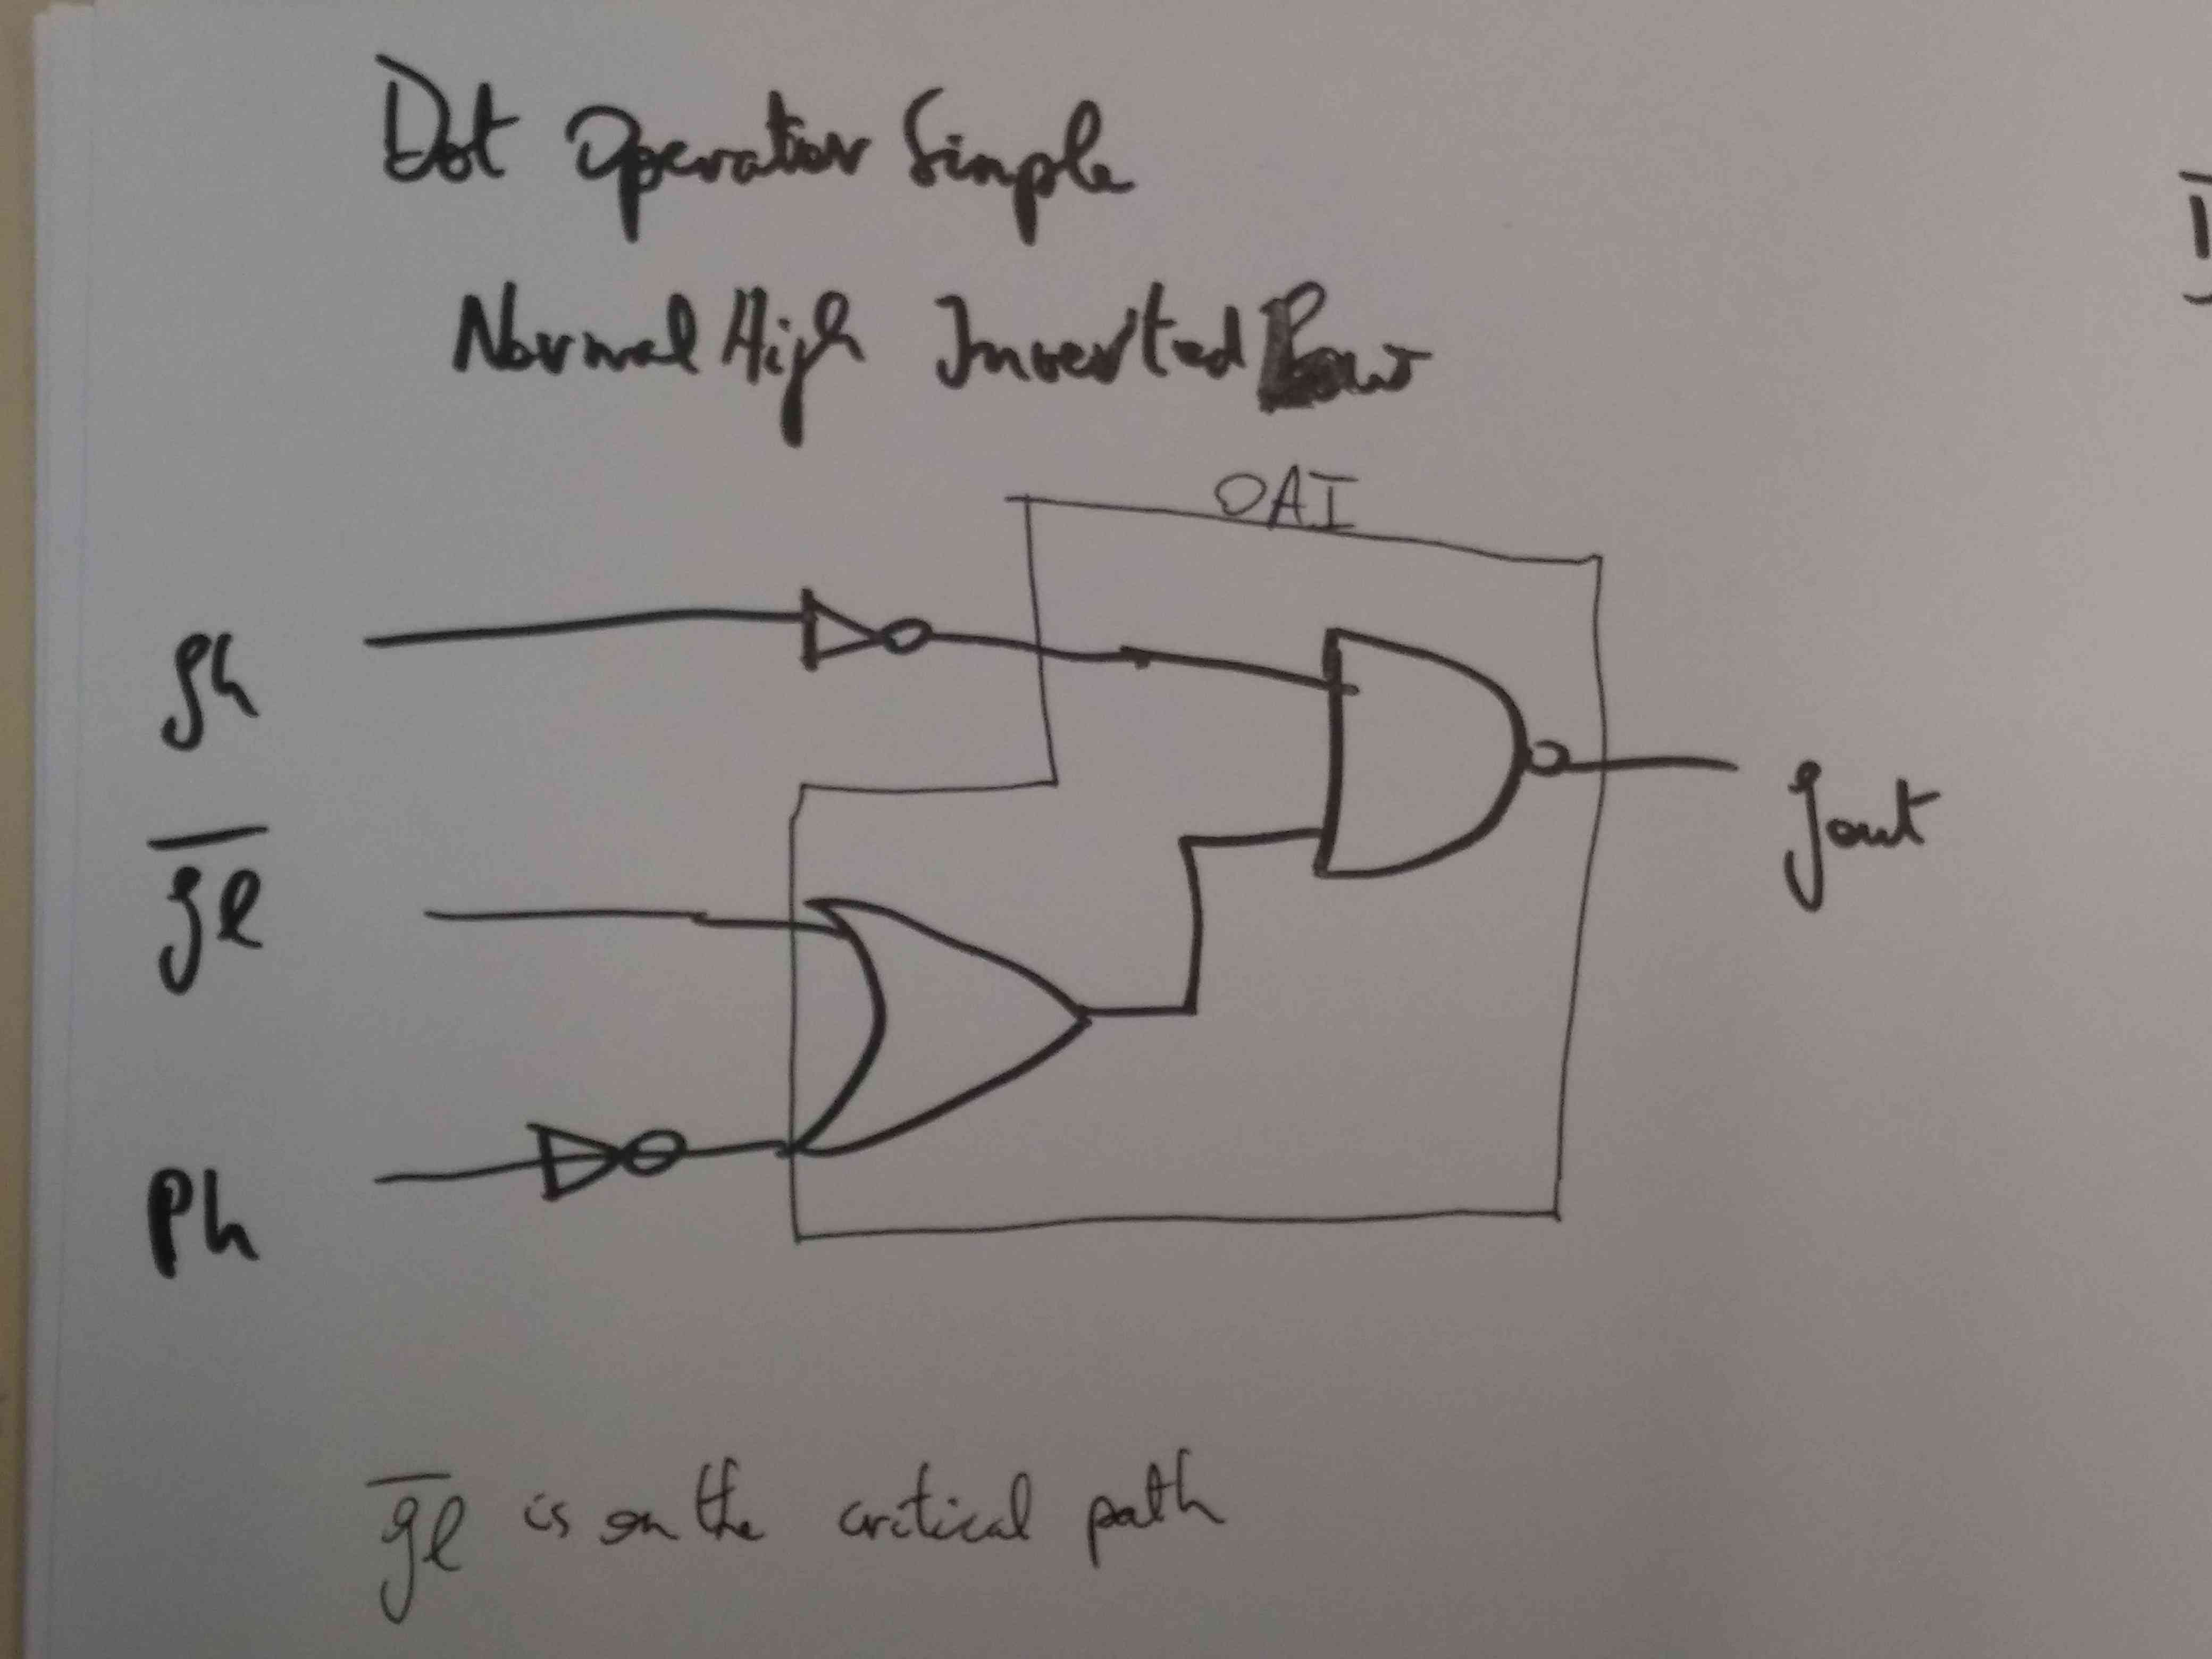
\includegraphics[width=0.9\textwidth]{figures/dosnhil}
\caption{the Dot Operator Simple \\Normal High inputs, Inverted Low inputs ('DOSNHIL')}
\label{DONHIL}
\end{subfigure}%
\begin{subfigure}{.5\textwidth}
  \centering
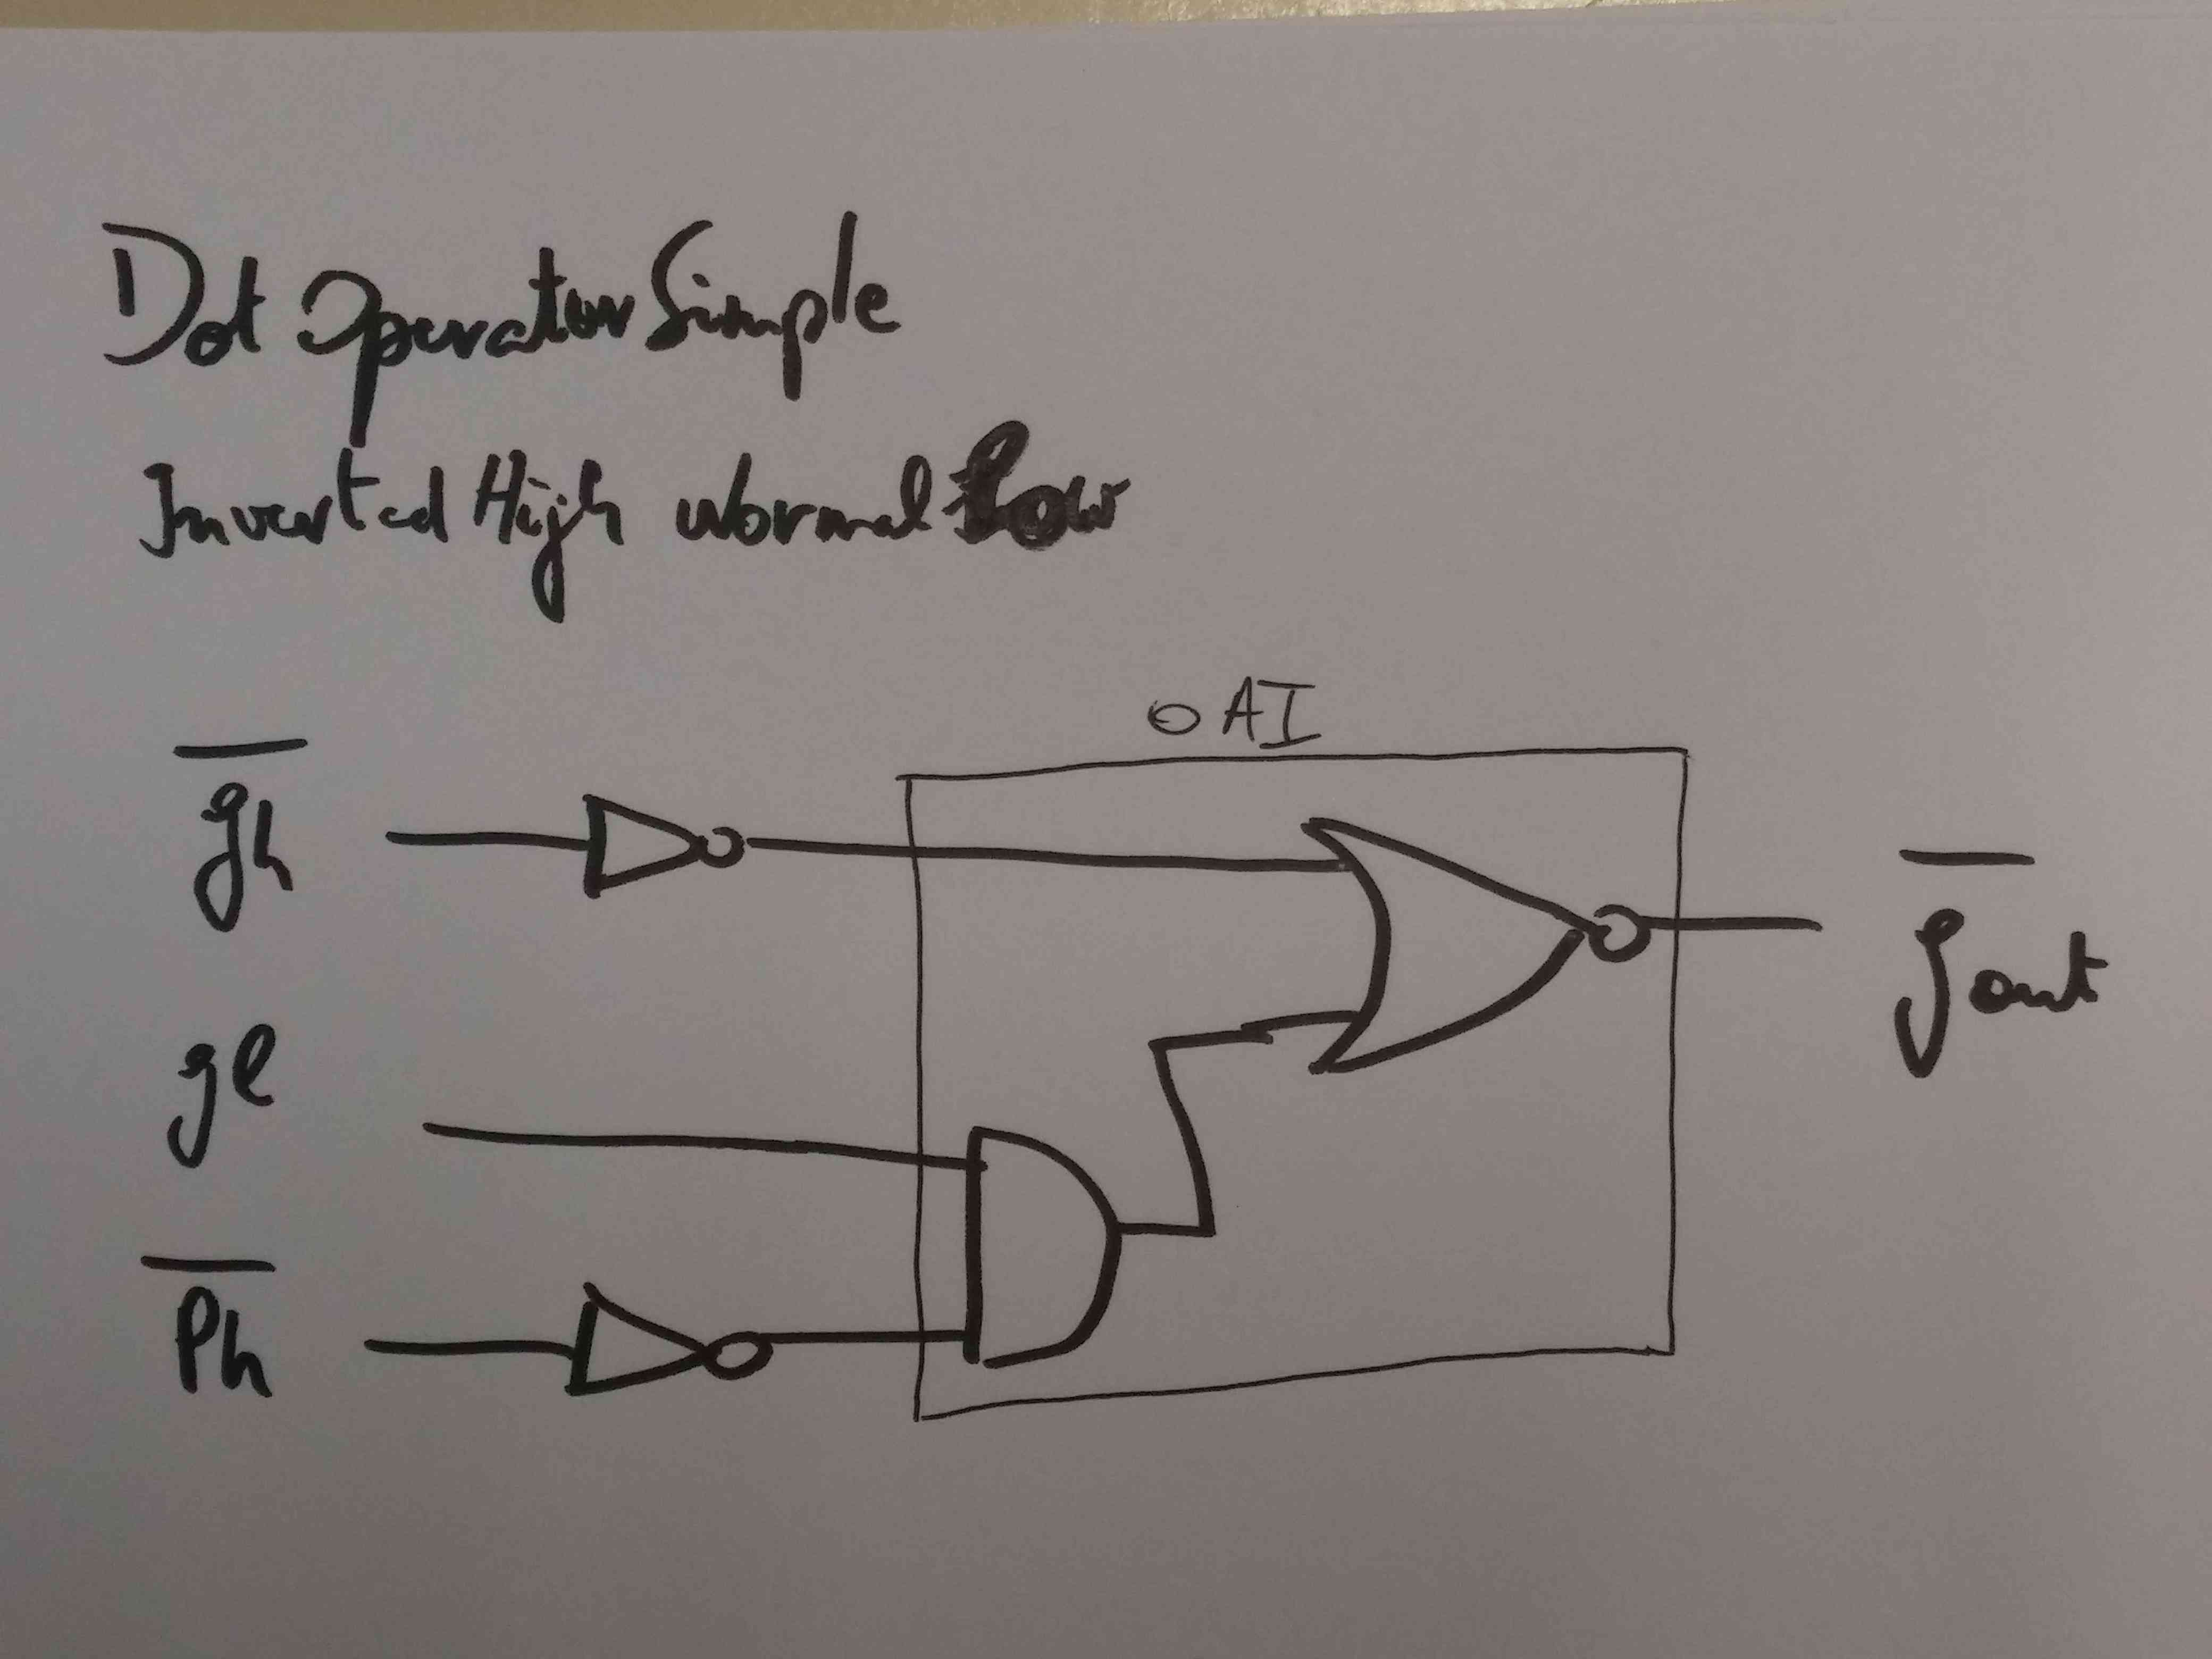
\includegraphics[width=0.9\textwidth]{figures/dosihnl}
\caption{Dot Operator Simple \\Inverted High inputs, Normal Low inputs ('DOSIHNL')}
\label{DONIHNL}
\end{subfigure}
\end{figure}

\subsubsection{Structural view}

\begin{figure}[H]
\begin{centering}
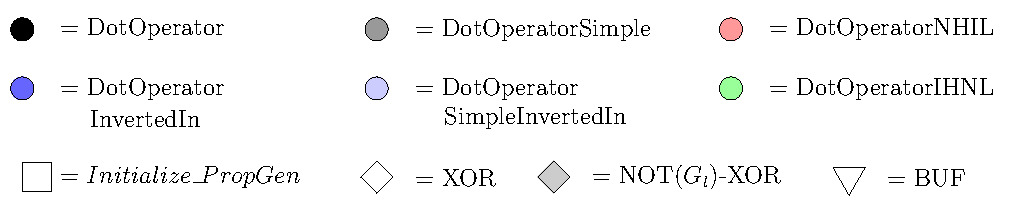
\includegraphics[width=0.9\textwidth, height=0.1\paperheight]{figures/adderLegend}
\par\end{centering}
\label{adderLegend}
\end{figure}

\begin{figure}[H]
\begin{centering}
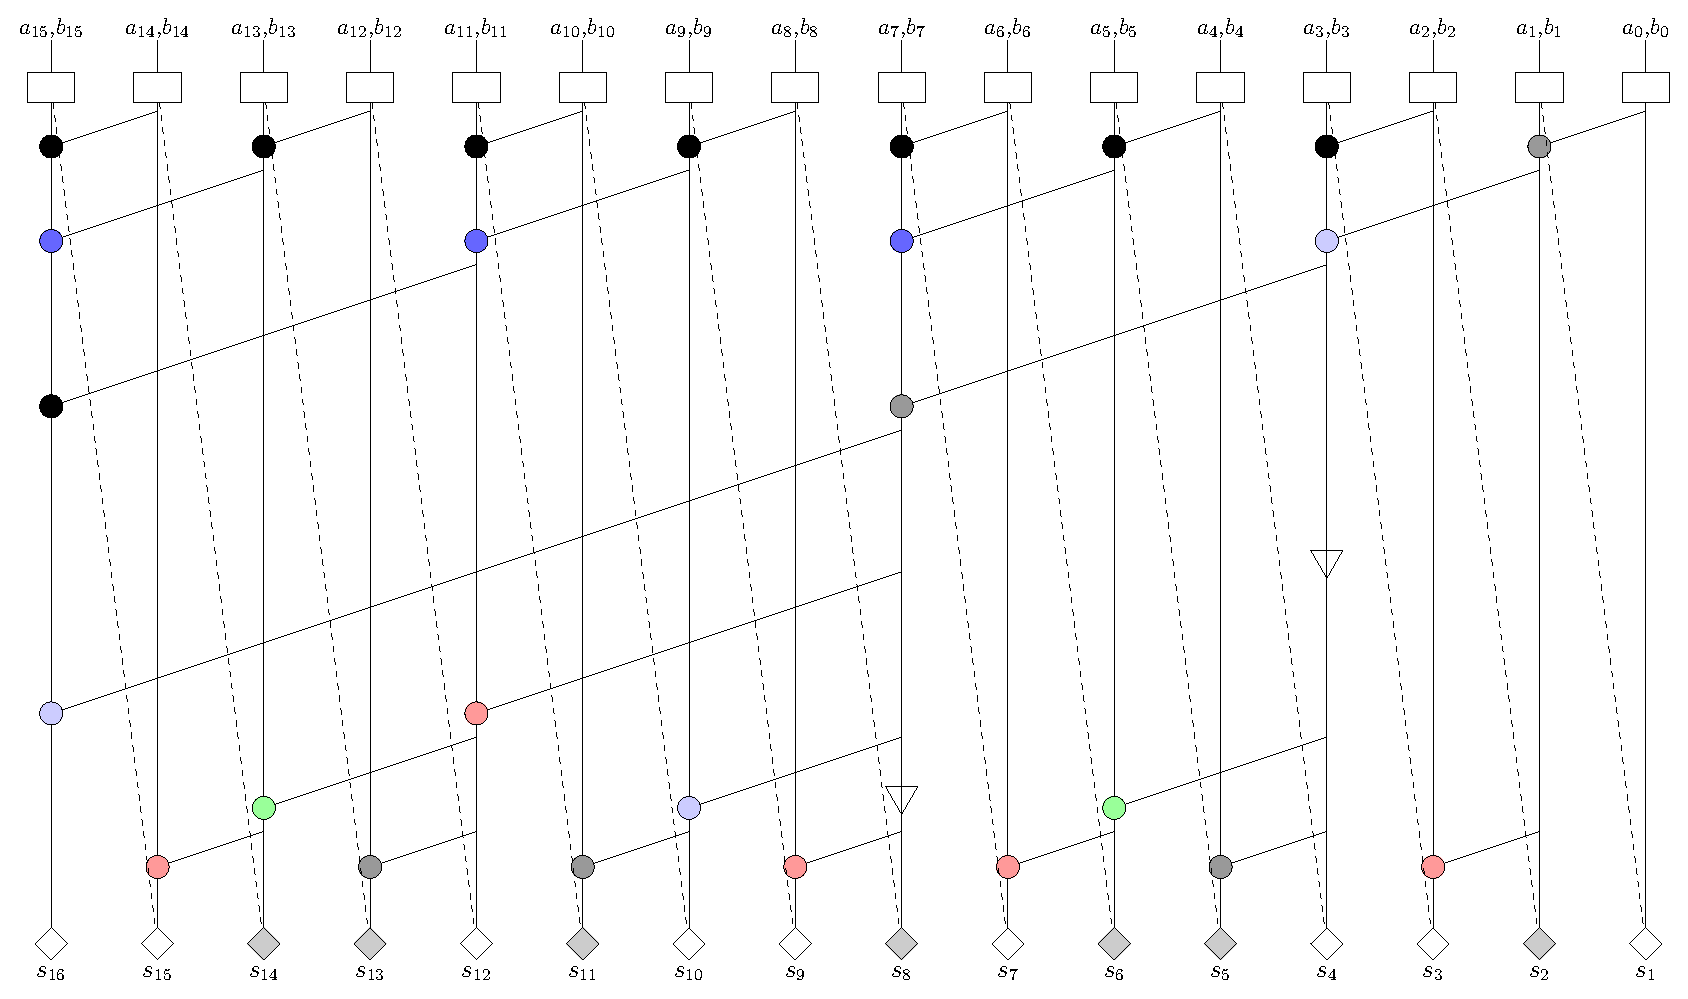
\includegraphics[angle=90,height=0.60\paperheight]{figures/adderStructure}
\par\end{centering}
\caption{Schematic of the optimised adder}
\label{adderSchematic}
\end{figure}

\subsubsection{Other performance metrics}
\begin{figure}[H]
\begin{centering}
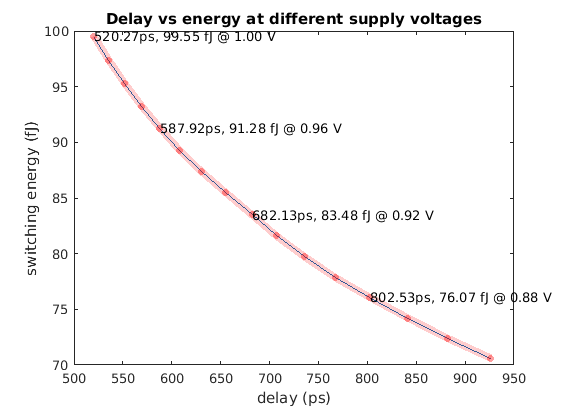
\includegraphics[width=0.9\textwidth]{figures/EDPlabeled.png}
\par\end{centering}
\caption{EDP of the optimised adder, for path to s15}
\label{adderEDP}
\end{figure}

\subsubsection{Other performance metrics}
\begin{figure}[H]
\begin{centering}
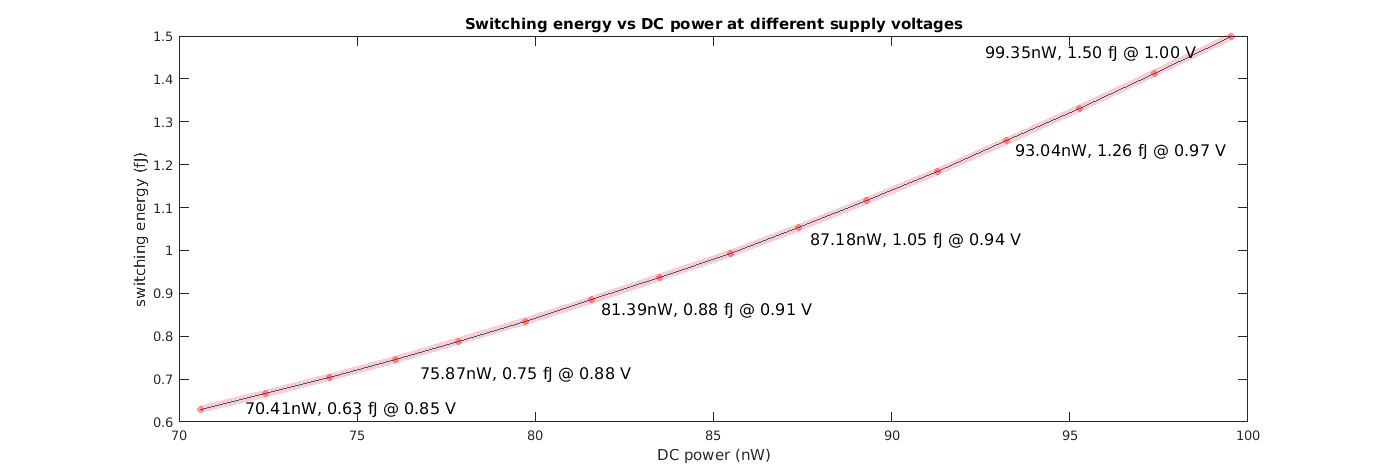
\includegraphics[width=0.9\textwidth]{figures/dynamicStaticEnergy.png}
\par\end{centering}
\caption{Dynamic switching energy vs static DC power consumption of the optimized adder}
\label{adderEDP}
\end{figure}

\medskip

\begin{thebibliography}{9}

\bibitem{website:xorTransmissionGate}
Universitat Hamburg
\textit{CMOS transmission-gate XOR gate}
accessed: 28/10/2016
\\\texttt{https://tams-www.informatik.uni-hamburg.de/applets/hades/webdemos/05-switched/40-cmos/xor-tgate.html}

\bibitem{adderOverview}
Noel Daniel Gundi
\textit{Implementation of 32 bit Brent-Kung adder using complementary pass transistor logic}
accessed: 28/10/2016
\\\texttt{https://shareok.org/bitstream/handle/11244/25747/Gundi\_okstate\_0664M\_13905.pdf?sequence=1}

\end{thebibliography}
 



\end{document}
